\chapter*{Übung 8}

\section*{Aufgabe 17}

Für eine Skizze der Aufgabe mit den Koordinaten siehe Abbildung \ref{fig:ueb8_aufgabe17}.

\begin{figure}[h]
	\centering
	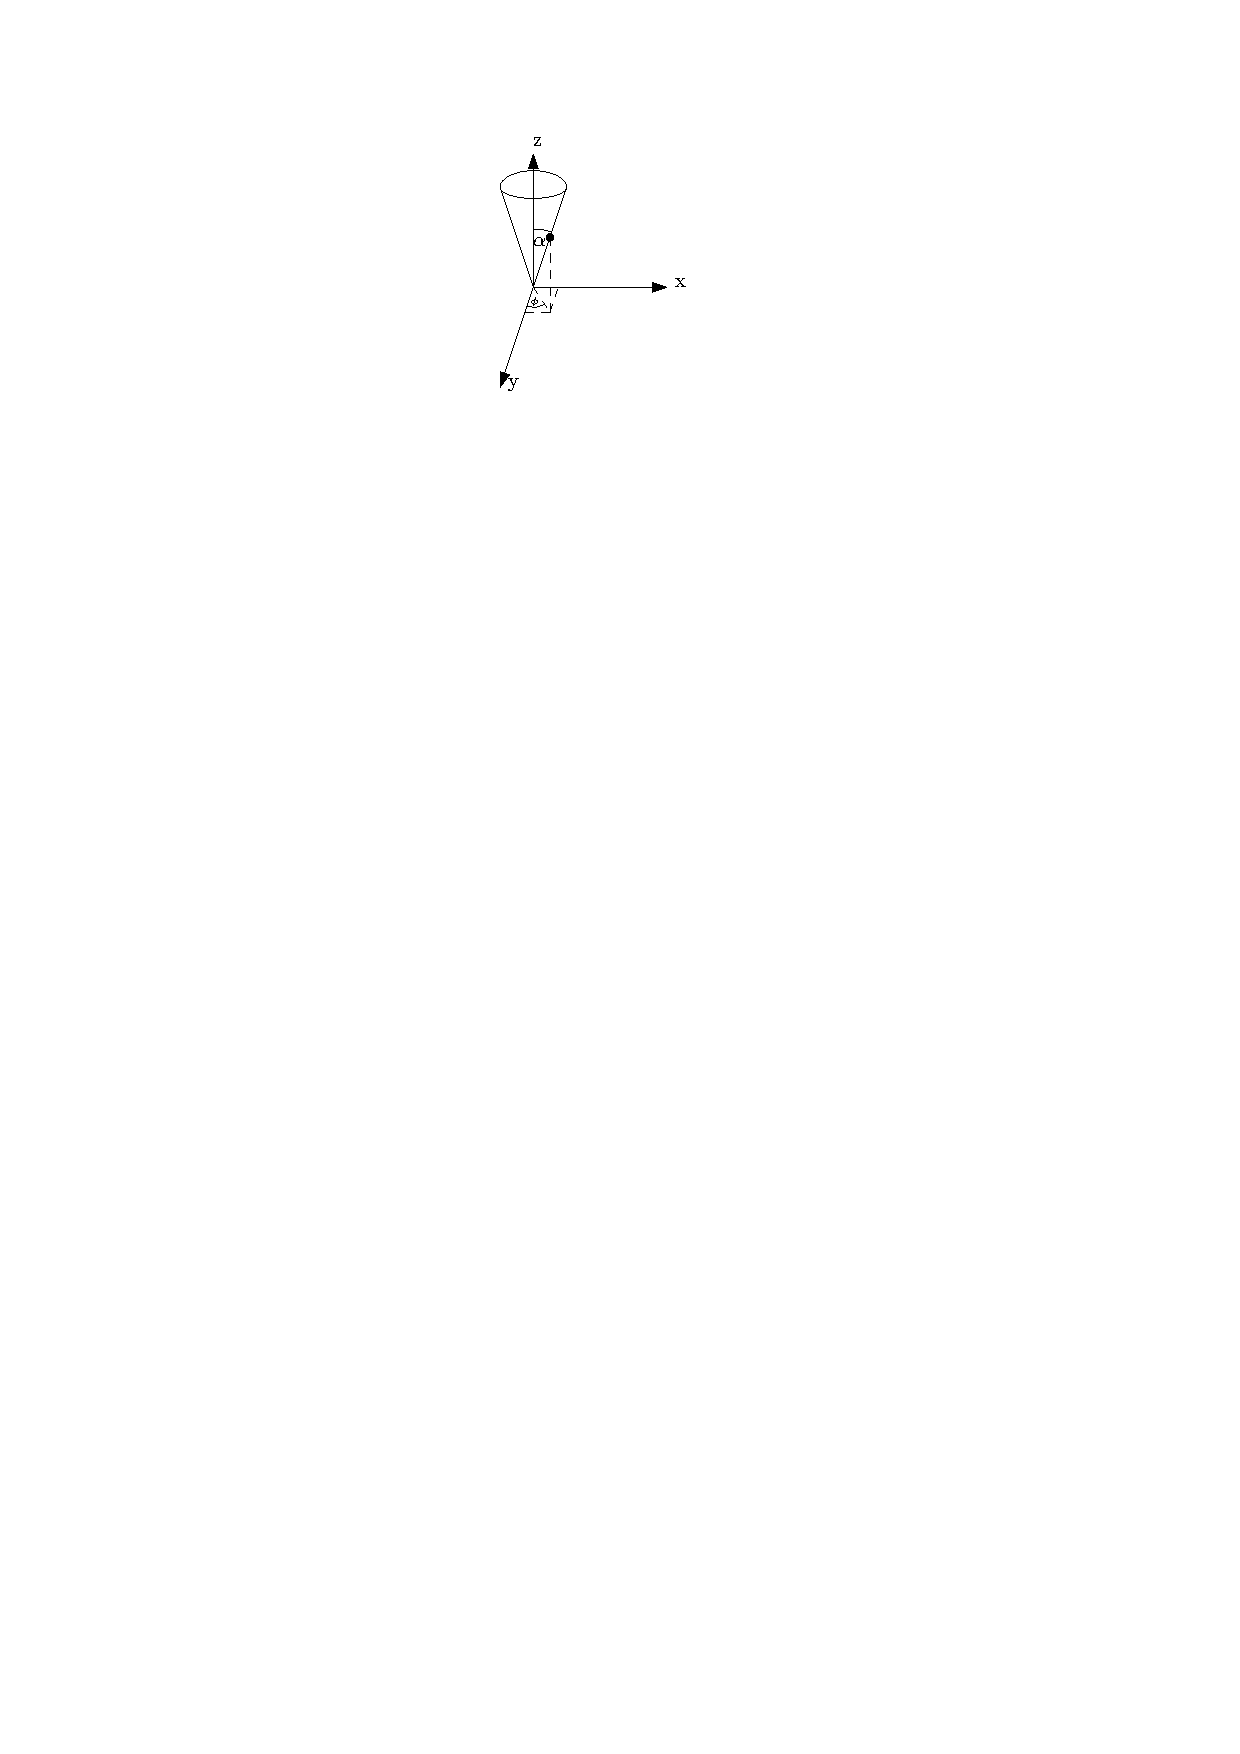
\includegraphics{figures/ueb8/aufgabe17}
	\caption{Skizze von Aufgabe 17 mit eingezeichneten Koordinaten.}
	\label{fig:ueb8_aufgabe17}
\end{figure}

Der Abstand der Masse zur $z$-Achse ist $r = \sqrt{x^2 + y^2}$ und der Zusammenhang zwischen Abstand und $z$-Koordinate ist $\tan(\alpha) = \frac{r}{z}$. Also ist die Zwangsbedingung $0 = \frac{\sqrt{x^2 + y^2}}{\tan(\alpha)} - z$.

Mit $r = z \tan(\alpha)$ ist dann
\begin{align*}
	x &= \sin(\phi) z \tan(\alpha) \text{,} \\
	y &= \cos(\phi) z \tan(\alpha) \text{,} \\
	\dot{x} &= \tan(\alpha) (\cos(\phi) \dot{\phi} z + \sin(\phi) \dot{z}) \text{,} \\
	\dot{y} &= \tan(\alpha) (\cos(\phi) \dot{z} - \sin(\phi) \dot{\phi} z) \text{,} \\
	V &= m g z \text{,} \\
	T &= \frac{1}{2} m (\dot{x}^2 + \dot{y}^2 + \dot{z}^2 ) \\
	  &= \frac{1}{2} m \left( \dot{z}^2 + \tan^2(\alpha) ( \sin^2(\phi) \dot{\phi}^2 z^2 + \cos^2(\phi) \dot{z}^2 + \cos^2(\phi) \dot{\phi}^2 z^2 + \sin^2(\phi) \dot{z}^2) \right) \\
	  &= \frac{1}{2} m \left( \dot{z}^2 (1 + \tan^2(\alpha)) + \tan^2(\alpha) \dot{\phi}^2 z^2 \right) \text{,} \\
	\mathcal{L} &= T - V = \frac{1}{2} m \left( \dot{z}^2 (1 + \tan^2(\alpha)) + \tan^2(\alpha) \dot{\phi}^2 z^2 \right) - m g z
\end{align*}

Nun stellen wir die Lagrange-Gleichung auf:
\[
	\msimplediff{}{t} \frac{\partial \mathcal{L}}{\partial \dot{q}_i} - \frac{\partial \mathcal{L}}{\partial q_i} = 0
\]

Für $\phi$ rechnen wir:
\begin{align*}
	&~ \msimplediff{}{t} \left( \frac{1}{2} 2 m \dot{\phi} z^2 \tan^2(\alpha) \right) - 0 = 0 \\
	\Longrightarrow &~ \msimplediff{}{t} (\dot{\phi} z^2) = 2 z \dot{\phi} \dot{z} + z^2 \ddot{\phi}) = 0 \\
	\Longrightarrow &~ \dot{\phi} \dot{z} + z \ddot{\phi} = 0
	\text{.}
\end{align*}

Für $z$ rechnen wir:
\begin{align*}
	&~ \msimplediff{}{t} (m \dot{z}^2 (1 + \tan^2(\alpha))) - m z \tan^2(\alpha) \dot{\phi}^2 + mg = 0 \\
	\Longrightarrow &~ \ddot{z} (1 + \tan^2(\alpha)) - z \dot{\phi}^2 \tan^2(\alpha) + g = 0
	\text{.}	
\end{align*}

Wir berechnen nun die Impulse:
\begin{align*}
	\mimpuls{\phi} &= \frac{\partial \mathcal{L}}{\partial \dot{\phi}} = m r^2 \dot{\phi} = m z^2 \tan^2(\alpha) \dot{\phi} \text{,} \\
	\mimpuls{z} &= \frac{\partial \mathcal{L}}{\partial \dot{z}} = m \dot{z} (\tan^2(\alpha) + 1)
	\text{.}	
\end{align*}

Umstellen nach den Koordinaten:
\begin{align*}
	\dot{\phi} &= \frac{1}{m r^2} P \phi = \frac{1}{m z^2 \tan^2(\alpha)} P \phi \text{,} \\
	\dot{z} &= \frac{1}{m (1 + \tan^2(\alpha))} P z \text{.}	
\end{align*}

Die Hamiltonfunktion lautet nun
\[
	H = \frac{1}{2m} \left( \frac{P \phi^2}{z^2 \tan^2(\alpha)} + \frac{P z^2}{1 + \tan^2(\alpha)} \right) + mgz \text{.}
\]

Wir berechnen weiter:
\begin{align*}
	\dot{\phi} &= \frac{\partial H}{\partial \mimpuls{\phi}} = \frac{1}{m} \frac{\mimpuls{\phi}}{z^2 \tan^2(\alpha)} \text{,} \\
	\dot{z} &= \frac{\partial H}{\partial \mimpuls{z}} = \frac{1}{m} \frac{\mimpuls{z}}{1 + \tan^2(\alpha)} \text{,} \\
	\dot{\mimpuls{\phi}} &= - \frac{\partial H}{\partial \phi} = 0 \text{,} \\
	\dot{\mimpuls{z}} &= - \frac{\partial H}{\partial z} = \frac{1}{m} \frac{\mimpuls{\phi}^2}{z^3 \tan^2(\alpha)} - mg \text{.}
\end{align*}

Damit überprüfen wir nun die Gleichungen von (a):
\[
	\ddot{\phi} = \frac{1}{m} \frac{\dot{\mimpuls{\phi}}}{z^2 \tan^2(\alpha)} - 2 \frac{1}{m} \dot{z} \frac{\mimpuls{\phi}}{z^3 \tan^2(\alpha)} = \frac{1}{m} \cdot 0 - 2 \frac{1}{m} \dot{z} \frac{1}{z} m \dot{\phi}
	\quad \Longrightarrow \quad 
	z \ddot{\phi} + 2 \dot{z} \dot{\phi} = 0 
	\text{.}
\]
Sowie:
\[
	\ddot{z} 
	= \frac{1}{m} \frac{\dot{\mimpuls{z}}}{1 + \tan^2(\alpha)} 
	= \frac{1}{m} \frac{1}{1 + \tan^2(\alpha)} \left( \frac{1}{m} \frac{\mimpuls{\phi}^2}{z^3 \tan^2(\alpha)} - mg \right)
	= \frac{1}{m} \frac{1}{1 + \tan^2(\alpha)} (m z \dot{\phi}^2 \tan^2(\alpha) - mg) \text{,}
\]
also $\ddot{z} (1 + \tan^2(\alpha)) - z \dot{\phi}^2 \tan^2(\alpha) + g = 0$.

Nun nehmen wir $z$ als konstant an, also $\dot{z} = \ddot{z} = 0$. Weiter ist wegen $z \ddot{\phi} = 0$ auch $\ddot{\phi} = 0$. Wir haben also eine Bewegung auf einer Kreisbahn. Nun berechnen wir $\dot{\phi}$ mit
\[
	z \dot{\phi}^2 \tan^2(\alpha) + g = 0
	\quad \Longleftrightarrow \quad 
	\dot{\phi}^2 = \frac{g}{z \tan^2(\alpha)}
	\quad \Longrightarrow \quad 
	\dot{\phi} = \sqrt{\frac{g}{z \tan^2(\alpha)}} 
	\text{.}
\]

Damit ergibt sich 
\[
	\phi(t) = \int \sqrt{\frac{g}{z \tan^2(\alpha)}} \md t + \phi_0 = \sqrt{\frac{g}{z \tan^2(\alpha)}} t + \phi_0
	\text{.}
\]

Das ist also die Winkelfunktion, die das Masseteilchen bräuchte, damit es sich auf einer Kreisbahn konstanter Höhe bewegt.

\section*{Aufgabe 18}

Die Lagrange-Funktion eines harmonischen Oszillators ist 
\[
	\mathcal{L} = \frac{1}{2} m \dot{x}^2 - \frac{1}{2} m \omega^2 x^2 \text{.}
\]

Nun führen wir folgende Transformation durch:
\[
	T: \quad \mvec{x' \\ \dot{x}' \\ t'} = \mvec{x + \alpha \cos(\omega t) \\ x - \alpha \omega \sin(\omega t) \\ t}
	\text{.}
\]

Das setzen wir zuerst in die Lagrange-Funktion ein und erhalten:
\begin{align*}
	L' &= \frac{1}{2} m \dot{x}^2 - \frac{1}{2} m \omega^2 x^2	 \\
	&= \frac{1}{2} m (\dot{x}' + \alpha \omega \sin(\omega t))^2
	   - \frac{1}{2} m \omega^2 (x' - \alpha \cos(\omega t))^2 \\
	&= \frac{1}{2} m \dot{x}^2 
	   + m \alpha \omega \dot{x} \sin(\omega t) 
	   + \frac{1}{2} m \alpha^2 \omega^2 \sin^2(\omega t)
	   - \frac{1}{2} m \omega^2 x^2 
	   + m \omega^2 \alpha x \cos(\omega t)
	   - \frac{1}{2} m \alpha^2 \omega^2 \cos^2(\omega t) \\
	&= \frac{1}{2} m \dot{x}^2 - \frac{1}{2} m \omega^2 x^2
	   - \frac{1}{2} m \alpha^2 \omega^2 (\cos^2(\omega t) - \sin^2(\omega t))
	   + m \omega \alpha (\dot{x} \sin(\omega t) + \omega x \cos(\omega t))
	\text{.}
\end{align*}

Vorgegeben ist nun $F(x', t, \alpha) = \alpha m \omega x' \sin(\omega t) + \alpha^2 f(t)$. Das leiten wir ab:
\[
	\msimplediff{}{t} F(x', t, \alpha) = \alpha^2 \dot{f}(t) + \alpha m \omega \dot{x}' \sin(\omega t) + \alpha m \omega^2 x' \cos(\omega t) \text{.}
\]

Wo wollen wir hin? Wir wollen nachrechnen, dass
\[
	\mathcal{L}'(x', \dot{x}', t; \alpha) = \mathcal{L}(x', \dot{x}', t) + \msimplediff{}{t} F(x', t; \alpha)
\]

Das geht, wenn wir 
\begin{align*}
	\dot{f}(t) 
	&= - \frac{1}{4} m \omega \left( 2 \omega (\cos^2(\omega t) - \sin^2(\omega t) \right) \\
	&= - \frac{1}{4} m \omega (2 \omega \cos(2 \omega t)) \\
	&= \msimplediff{}{t} \left( - \frac{1}{4} m w \sin(2 \omega t) \right)
\end{align*}
setzen.

Das in $F$ eingesetzt:
\[
	F(x', t, \alpha) = \alpha m \omega x' \sin(\omega t) - \frac{1}{4} m \omega \alpha^2 \sin(2 \omega t)
	\text{.}
\]

Wichtig: Nur weil man diese Funktion eindeutig definieren kann, kann man feststellen, dass es sich um eine Symmetrietransformation handelt.

Nun berechnen wir den Strom zu
\begin{align*}
	J
	&= \frac{\partial \mathcal{L}}{\partial \dot{x}} \left. \frac{\partial x(x', t, \alpha)}{\partial \alpha} \right|_{\alpha = 0} - \left. \frac{\partial F}{\partial \alpha} \right|_{\alpha = 0} \\
	&= \frac{\partial \mathcal{L}}{\partial \dot{x}} \left. \frac{\partial (x' - \alpha \cos(\omega t))}{\partial \alpha} \right|_{\alpha = 0} - \left. \frac{\partial F}{\partial \alpha} \right|_{\alpha = 0} \\
	&= m \dot{x} (- \cos(\omega t) - \left( m \omega x' \sin(\omega t) - \frac{1}{2} m \omega \alpha \sin(2 \omega t) \right)_{\alpha = 0} \\
	&= - m \dot{x} \cos(\omega t) - m \omega x' \sin(\omega t) \\
	&= - m ( \dot{x} \cos(\omega t) + \omega x' \sin(\omega t) )	 \text{.}
\end{align*}

Nun zu (b). Es ist 
\begin{align*}
	H &= \frac{1}{2} m \dot{x}^2 + \frac{1}{2} m \omega^2 x^2 = \frac{1}{2} \frac{p^2}{m} + \frac{1}{2} m \omega^2 x^2 \text{,} \\
	\dot{x}	&= [x, H] = \frac{\partial x}{\partial x} \frac{\partial H}{\partial p} - \frac{\partial H}{\partial x} \frac{\partial x}{\partial p} = \frac{\partial H}{\partial p} = \frac{p}{m} \text{,} \\
	\dot{p} &= [p, H] = \frac{\partial p}{\partial x} \frac{\partial H}{\partial p} - \frac{\partial H}{\partial x} \frac{\partial p}{\partial p} = - \frac{\partial H}{\partial x} = - m \omega^2 x \text{.}
\end{align*}

Weiter berechnen wir
\begin{align*}
	A &= - m (\dot{x} \cos(\omega t) + \omega x \sin(\omega t)) = - p \cos(\omega t) - m \omega x \sin(\omega t) \text{,} \\
    [A, H] &= \left[ -p \cos(\omega t) - m \omega x \sin(\omega t), 	\frac{p^2}{2m} + \frac{1}{2} m \omega^2 x^2 \right] \\
	       &= \frac{\partial A}{\partial x} \frac{\partial H}{\partial p} - \frac{\partial H}{\partial x} \frac{\partial A}{\partial p} \\
	       &= m \omega \sin(\omega t) \frac{p}{m} + m \omega^2 x \cos(\omega t) \text{,} \\
	\frac{\partial A}{\partial t} &= p \omega \sin(\omega t) - m \omega^2 x \cos(\omega t) \text{.}
\end{align*}

Da also
\[
	\frac{\md A}{\md t} = [A, H] + \frac{\partial A}{\partial t} = 0
\]
ist $A$ eine Erhaltungsgröße.

